\begin{frame}
\frametitle{Method}
\framesubtitle{Adding Conditioning Input}
\begin{figure}
    \centering
    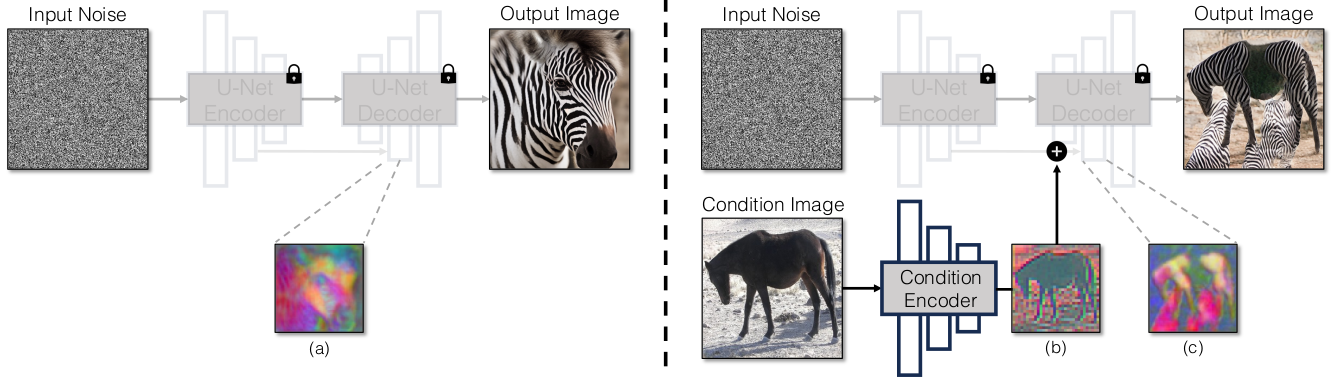
\includegraphics[width=1\linewidth]{images/Bildschirmfoto vom 2024-04-14 10-57-39.png}
    \caption{Conflicts between noise and conditional input}
\end{figure}
\end{frame}
\note{
    Methoden-Teil:\\
    \begin{enumerate}
        \item Text-to-image Model was für Image translation verwendet werden soll
        \item Problem von detail verlust bei der Übersetzung wie das umgangen werden kann
        \item Unpaired image translation
        \item Architecture Änderungen für Paired image Translation
    \end{enumerate}
    \textbf{RESTLICHEN NOTIZEN SIEHE ZETTEL}
    
}

% ---------- Preserving Input Details ----------
\begin{frame}
\frametitle{Method}
\framesubtitle{Preserving Input Details}
\begin{figure}
    \centering
    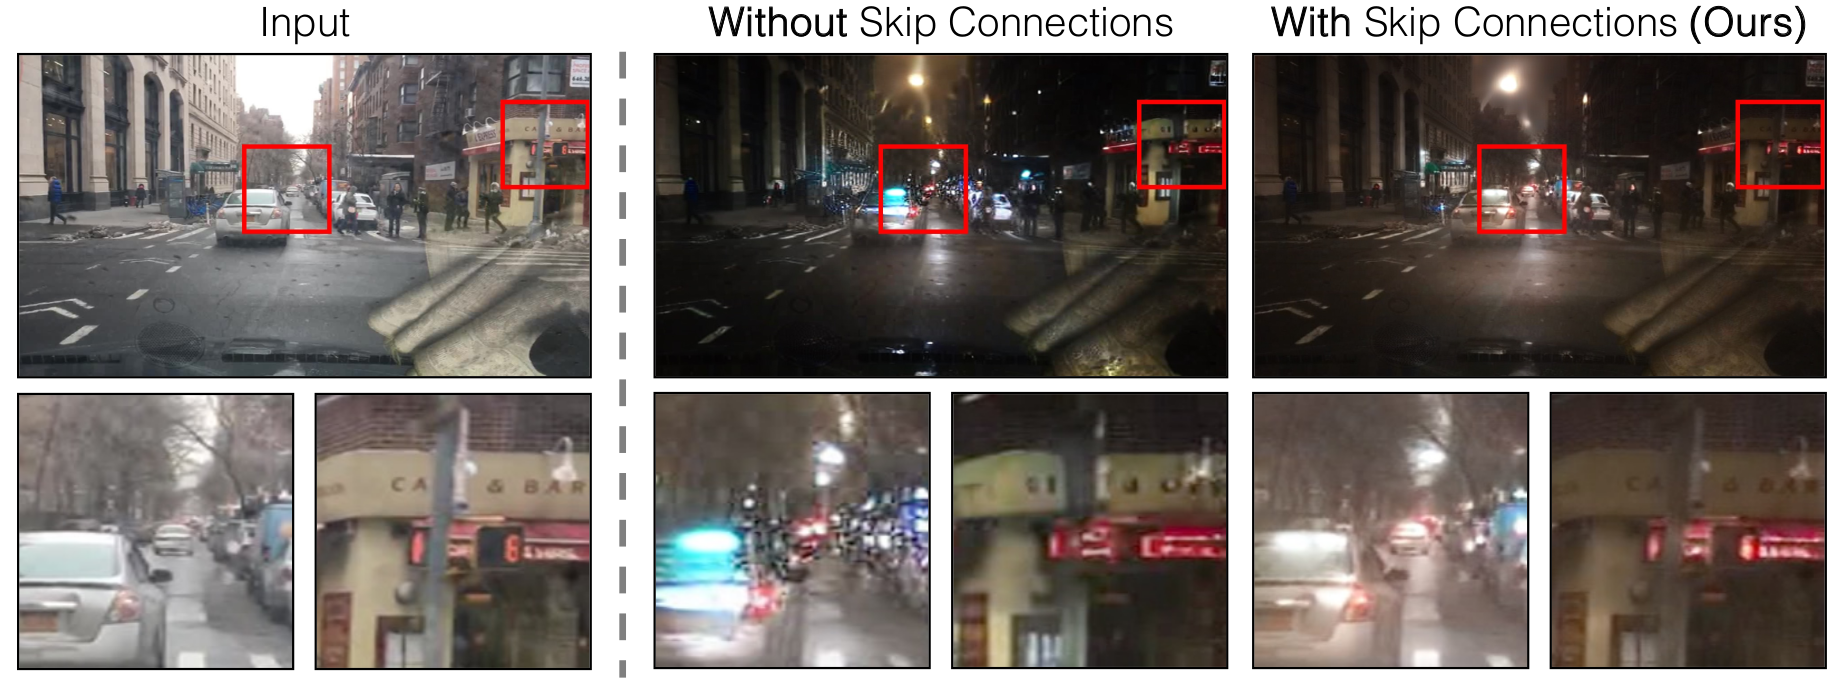
\includegraphics[width=0.9\linewidth]{images/Bildschirmfoto vom 2024-04-14 11-06-40.png}
    \caption{Skip Connections help retain details}
\end{figure}
\end{frame}
\note{
    Warum gehen Details verloren?\\
    \begin{itemize}
        \item Die Bild Encoder von Latent Diffusion Modellen komprimieren Inputbilder um das 8fache und erhöhen die Dimension von 3 auf 4
        \item So wird zwar Training und Inference von Diffusion Modellen schneller, ist aber nicht ideal für Image Translation, wo man details erhalten will
    \end{itemize}
    Wie können Details erhalten werden?\\
    \begin{itemize}
        \item Um Details zu erhalten werden Skip Connections zwischen Encoder und Decoder eingeführt
        \item Nach jedem Downsampling Schritt im Encoder wird eine 1x1 zero-convolution schicht durchlaufen und an die entsprechende Schicht im Decoder weitergegeben
    \end{itemize}
    Siehe Bild, links der Input, Mitte ohne Skip Connections, rechts mit Skip Connections\\
    Ohne Skip Connections verschwindet das Auto in der Ferne und der Text ist nicht lesbar
}


% ---------- Preserving Input Details ----------
\begin{frame}
\frametitle{Method}
\framesubtitle{Preserving Input Details}
\begin{figure}
    \centering
    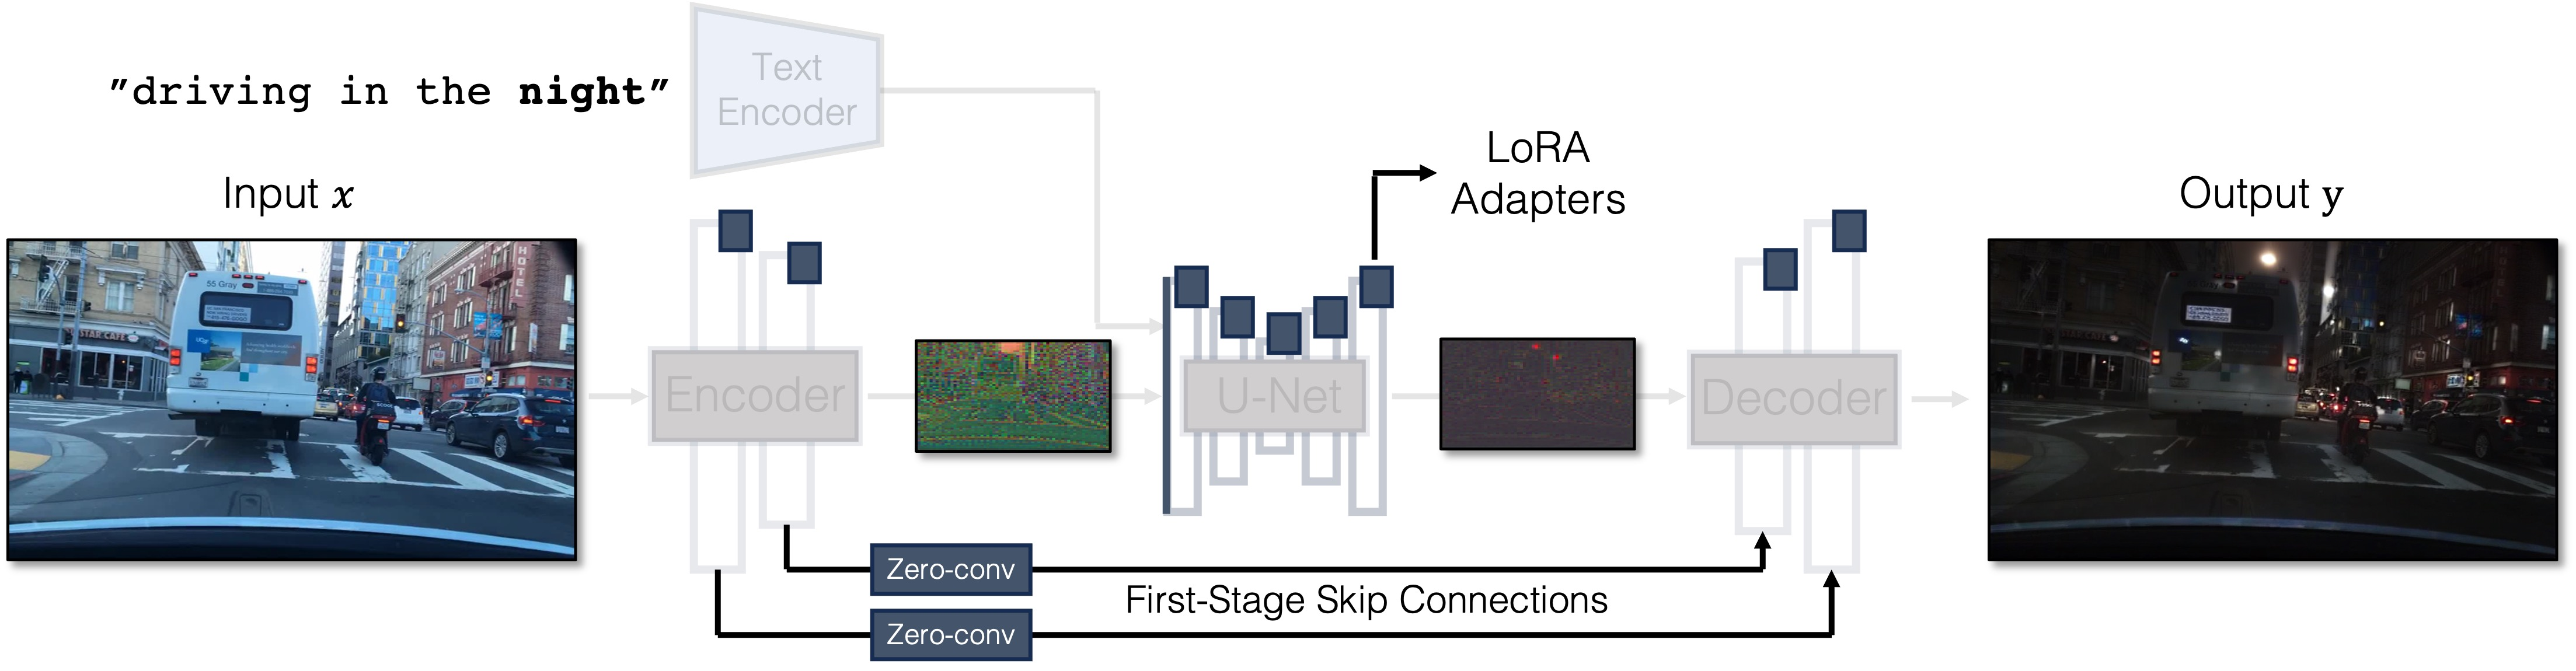
\includegraphics[width=1\linewidth]{images/method.jpg}
    \caption{Model Architecture}
\end{figure}
\end{frame}
\note{
    Die Architecture besteht im wesentlichen aus 4 Teilen:
    \begin{enumerate}
        \item Einem Text Encoder und einem Bild Encoder für den Input
        \item Das vortrainierte Stable Diffusion Model
        \item Und einem Decoder
        \item Der Text Encoder, Bild Encoder und Decoder stammen alle aus dem StableDiffuion Model
        \item In das Model und dem Encoder und Decoder wurden auf jeder Ebene LoRA Gewichte eingeführt
        \item Die erste schicht des Stable Diffusion wird neu trainiert
        \item Und es werden 1x1 zero-convolution Skip Connecitons zwischen Encoder und Decoder eingeführt
        \item Kurz gesagt, alles was Blau ist wurde neu trainiert, alles was grau ist bleibt unverändert
    \end{enumerate}
}


% ---------- Unpaired Training ----------
\begin{frame}
    \frametitle{Method}
    \framesubtitle{Unpaired Training}
    \begin{align*}
    \text{Goal:} &\text{ Convert images from } \mathcal{X} \subset \mathbb{R} ^{H \times W \times 3} \
    \text{ to } \mathcal{Y} \subset \mathbb{R} ^{H \times W \times 3} \\
    &\text{ given an unpaired dataset } \mathcal{X} = {x \in \mathcal{X} } \text{ and } \mathcal{Y} = {y \in \mathcal{Y} } \\
    &\text{ using one network } G \text{ and two translations } G(x, c_y): \mathcal{X} \rightarrow \mathcal{Y} \
    \text{ and } G(y, c_x): \mathcal{Y} \rightarrow \mathcal{X}
    \end{align*}
\end{frame}
\note{
    Ziel ist es Bilder von der Domain X in Domain Y zu übersetzen.\\
    Bei zwei gegebenen unpaired Datensätzen X und Y\\
    Und das ganze mit dem gleichen Netzwerk G\\
    Die Notation $G(x,c_y)$ bedeutet, dass das Netzwerk x in y übersetzt, wobei $c_y$ eine Übersetzungsaufgabe darstellt z.B. Tag -> Nacht
}


\begin{frame}
\frametitle{Method}
\framesubtitle{Unpaired Training}
\begin{block}{Cycle consistency with perceptual loss}
    \begin{equation}
        \mathcal{L}_{\text{cycle}}(G, F) = \mathbb{E}_x [ \mathcal{L}_\text{rec} (G(G(x,c_Y), c_X), x) ] + \mathbb{E}_y [ \mathcal{L}_\text{rec} (G(G(y,c_X), c_Y), y) ]
    \end{equation}
\end{block}
with $\mathcal{L}_{\text{rec}}$ as combination of L1 and LPIPS \cite{zhang2018unreasonable}
\begin{block}{Adversarial loss}
    \begin{align}
        \mathcal{L}_{\text{GAN}} &= \mathbb{E}_{y} [\log D_Y(y)] + \mathbb{E}_{x} [\log(1 - D_Y(G(x,c_Y)))] \\
        &+ \mathbb{E}_{x} [\log D_X(x)] + \mathbb{E}_{Y} [\log(1 - D_X(G(y,c_X)))]
    \end{align}
\end{block}
\end{frame}
\note{
    Cycle Consistency loss: \\
    \begin{itemize}
        \item Die Cycle Consistency Loss Funktion sorgt dafür, dass die Übersetzung von x nach y und wieder zurück das Originalbild x ergibt
        \item $\mathcal{L}_{\text{rec}}$ ist eine Kombination aus L1 und LPIPS Loss
        \item LPIPS steht für Learned Perceptual Image Patch Similarity und ist ein Maß für die Ähnlichkeit von Bildern. Das Maß ist vergleichbar mit menschlicher Wahrnehmung

    \end{itemize}
    Adversarial loss: \\
    \begin{itemize}
        \item Der Adversarial loss sorgt dafür, dass die Übersetzung von x nach y bzw. von y nach x möglichst der Ziel Domain entspricht.
        \item Hier zu werden zwei Discriminatoren $D_x$ und $D_y$, um Übersetzte Bilder von Realen zu unterscheiden
        \item Die Discriminatoren nutzen hierfür beide das CLIP Modell(Contrastive Language-Image Pre-training)
    \end{itemize}
}


\begin{frame}
\frametitle{Method}
\framesubtitle{Unpaired Training}
\begin{block}{Identity regularization loss}
    \begin{equation}
        \mathcal{L} _{\text{idt}} = \mathbb{E} _y [ \mathcal{L}_{\text{rec}}(G(y,c_Y),y)] + \mathbb{E}_x [ \mathcal{L}_{\text{rec}}(G(x,c_X),x)]
    \end{equation}
\end{block}


\begin{block}{Full objective}
    \begin{equation}
        \arg \underset{G}{\min} \mathcal{L}_{\text{cycle}} + \lambda _{\text{idt}} \mathcal{L}_{\text{idt}} + \lambda_{\text{GAN}}\mathcal{L}_{\text{GAN}}
    \end{equation}
\end{block}
\end{frame}
\note{
    Identity Regularization loss: hilft dabei, dass Inhalte aus dem Inputbild bei der Übersetzung nicht verloren gehen.\\
    Full Objective: Die Gesamtverlustfunktion setzt sich aus den drei Verlustfunktionen zusammen.\\

}


% ---------- Extensions ----------
\begin{frame}
\frametitle{Method}
\framesubtitle{Extensions - Paired Training}
\begin{itemize}
    \item Adaptation of network G to paired setting, like edge-to-image or sketch-to-image, called pix2pix-Turbo
    \item new translation function $G(x,c): X \rightarrow Y$ where $X$ is source domain, $Y$ target domain and $c$ conditioning input
\end{itemize}
\begin{block}{Loss Function}
    \begin{equation}
        \arg \underset{G}{\min} \mathcal{L}_{\text{rec}}+ \lambda _{\text{clip}}\mathcal{L}_{\text{CLIP}}+ \lambda_{\text{GAN}}\mathcal{L}_{\text{GAN}}
    \end{equation}
\end{block}
\end{frame}
\note{
    Der Fokus des Papers liegt zwar auf unpaired Image Translation, aber es gibt auch eine Erweiterung für paired Image Translation.\\
    Dieser Abschnitt befasst sich mit der Anpassung des Netzwerks G an ein gepaartes Setting, wie z.B. Kanten-zu-Bild oder Skizze-zu-Bild, genannt pix2pix-Turbo.\\
    Die neue Übersetzungsfunktion $G(x,c): X \rightarrow Y$ wobei $X$ die Quelldomäne, $Y$ die Ziel-Domäne und $c$ die Konditionierungseingabe ist.\\
    Die neue Verlustfunktion setzt sich aus der Rekonstruktionsverlustfunktion, dem CLIP text-image alignment Verlust und dem GAN-Verlust zusammen.\\
    GAN-Verlust und Rekonstruktionsverlust sind die gleichen wie im unpaired Setting\\
    CLIP text-image alignment Verlust ist ein Maß für die Ähnlichkeit von Bildern und Texten
}


\begin{frame}
    \frametitle{Method}
    \framesubtitle{Extensions - Generating diverse output}
    Introduction of interpolation coefficient $\gamma$ \newline 
    Three changes to the Architecture (1/3):
    \begin {itemize}
        \item Generator function $G(x,z,\gamma)$ combines noise z and encoder output like so: $\gamma G_{\text{enc}}(x) + (1 - \gamma) z$
        \item Output as U-Net input
    \end{itemize}
\end{frame}
\note{
    Zur Generierung von diversen outputs wir eine Interpolationskoeffizient $\gamma$ eingeführt.\\
    Desweiteren werden drei Änderungen an der Architektur vorgenommen.\\
    1. $gamma$ wird in die Generatorfunktion eingeführt.\\
    2. Der Output wird als U-Net Input verwendet
}


\begin{frame}
    \frametitle{Method}
    \framesubtitle{Extensions - Generating diverse output}
    Three changes to the Architecture (2/3):
    \begin {itemize}
        \item Scale LoRA weights and skip connections according to $\theta = \theta_0 + \gamma \Delta \theta$  
        \item where $\theta_0$ and $\Delta \theta$ denote the original weights and new weights.
    \end{itemize}
\end{frame}
\note{
    Skalierung von LoRA Gewichte und Outputs von Skip Connections neu gewichten
}


\begin{frame}
    \frametitle{Method}
    \framesubtitle{Extensions - Generating diverse output}
    Three changes to the Architecture (3/3):
    \begin {itemize}
        \item Scale reconstruction loss according to $\gamma$: $\mathcal{L}_{\text{diverse}} = \mathcal{L}_{x,y,z,\gamma} \gamma\mathcal{L}_{\text{rec}}(G(x,z,\gamma),y)]$
        \item $\gamma = 0$ corresponds to default stochastic behavior of pretrained model, in this case reconstruction loss is not enforced
        \item $\gamma = 1$ corresponds to deterministic translation from previoues seections
    \end{itemize}
\end{frame}
\note{
    Rekonstruktionsverlust wird nach $\gamma$ skaliert.\\
    $\gamma = 0$ entspricht dem Standardverhalten des vortrainierten Modells, in diesem Fall wird der Rekonstruktionsverlust nicht durchgesetzt.\\
    $\gamma = 1$ entspricht der deterministischen Übersetzung aus den vorherigen Abschnitten
}
